\documentclass{Interspeech}
\usepackage{amsmath,amssymb}
\usepackage{graphicx}
\usepackage{booktabs}
\usepackage{multirow}
\usepackage{url}
\usepackage{cite}

\title{Speaker Identity Is Split Across Conditioning Sites:\\
Prompt and Embedding Pathways in Zero-Shot Voice Cloning}

% Review mode (double-blind) is the default for Interspeech.cls.
\keywords{voice cloning, zero-shot TTS, speaker conditioning, in-context learning, speaker embedding}

\begin{document}
\maketitle

\begin{abstract}
Zero-shot voice-cloning systems condition on a target speaker through two routes at once: an in-context acoustic prompt and a global speaker embedding, which some systems inject into the language model and others only into the acoustic decoder. We remove the prompt while keeping the embedding in six open-weight systems on two test sets (25{,}509 utterances), and run a within-model factorial in CosyVoice that switches the prompt, the language-model embedding and the decoder embedding on and off independently (6{,}480 utterances). Across systems, identity survives prompt removal best when the embedding also conditions the language model. Within CosyVoice, the two embedding sites contribute additively to speaker similarity (about 0.10 and 0.19 SIM-o without the prompt), and the prompt can stand in for the language-model embedding but not for the decoder embedding. Dropping the prompt also stops the model reproducing the prompt's recording conditions, which raises predicted naturalness most for noisy prompts; we show this metric also rewards losing speaker identity.
\end{abstract}

%----------------------------------------------------------------------
\section{Introduction}
\label{sec:intro}
%----------------------------------------------------------------------

Zero-shot text-to-speech (TTS) clones a voice from seconds of reference audio~\cite{valle,seedtts,voicebox,qwen3tts}.
Most current systems condition on the reference in two ways at once: an \emph{acoustic prompt}, i.e.\ reference speech tokens or features placed in context, and a \emph{global speaker embedding} from a speaker encoder~\cite{cosyvoice,cosyvoice2,cosyvoice3,xtts}.
The two routes are rarely separated, so it is unclear which one carries speaker identity and which one carries everything else in the recording.
The distinction matters in practice: prompts are known to import their acoustic environment~\cite{lu2025noise,wang2024noise}, and prompt-free conditioning is attractive for privacy-preserving, streaming and cross-lingual use.

We isolate the routes by removing prompt-level conditioning while keeping each system's speaker embedding, in six open-weight systems that place the embedding at different depths.
Our contributions are:
\begin{enumerate}
  \item A matched prompt-removal study across six systems and two test sets, scored with the Seed-TTS-eval protocol and speaker-level statistics.
  \item A cross-system pattern: systems whose \emph{language model} also receives the embedding keep more identity without the prompt than systems that inject it only into the \emph{acoustic decoder}.
  \item A within-model causal factorial showing that the language-model and decoder embedding sites contribute additively to identity, and that the prompt substitutes for the language-model site but not for the decoder site.
  \item Evidence that prompts transfer recording conditions, and that the predicted-naturalness gain from dropping them partly reflects a metric that favours generic voices.
  \item A reference-count analysis: three references raise similarity by 0.02--0.04 in both routes without changing naturalness, while a prompt-only system (F5-TTS) degrades.
\end{enumerate}

%----------------------------------------------------------------------
\section{Related Work}
\label{sec:related}
%----------------------------------------------------------------------

\textbf{Speaker conditioning.}
VALL-E~\cite{valle} and F5-TTS~\cite{f5tts} rely only on an acoustic prompt, and StyleTTS~2~\cite{styletts2} only on a style embedding.
CosyVoice~\cite{cosyvoice} conditions both its language model and its flow decoder on an x-vector; CosyVoice~2 and~3~\cite{cosyvoice2,cosyvoice3} removed it from the language model, a change their developers describe as an interface redesign~\cite{chen2026bottleneck} but whose effect on identity has not, to our knowledge, been evaluated.
Comparisons of speaker encoders~\cite{yourtts} vary the embedding, not the route.

\textbf{Prompts and references.}
Longer or multiple prompts help when the architecture is trained for them~\cite{megatts2,lei2023multiscale,pfluxtts}.
Prompt noise propagates into the output of LLM- and flow-based TTS~\cite{lu2025noise,wang2024noise}, and robustness benchmarks probe noisy references across many systems~\cite{rvcbench}.
None of these separates the prompt from the embedding within a system, which is the comparison we make.

%----------------------------------------------------------------------
\section{Method}
\label{sec:method}
%----------------------------------------------------------------------

\subsection{Systems and the prompt-removal intervention}
\label{sec:systems}

Table~\ref{tab:systems} lists the systems.
In the \emph{full} condition each system receives its normal prompt and embedding from the reference.
In the \emph{x-vector only} condition we remove all prompt-level conditioning and keep the embedding: Qwen3-TTS's native \texttt{x\_vector\_only} mode~\cite{qwen3tts}; for CosyVoice and CosyVoice~3 we drop the prompt speech tokens and features from both the language model and the flow decoder; for XTTS-v2 we replace the GPT conditioning latents with a fixed mean over two held-out speakers; for Chatterbox we drop the T3 speech-prompt tokens.
Where the embedding enters was verified in each system's released inference code.
The interventions are system-specific, so we compare the \emph{pattern} across systems rather than treating them as identical.
F5-TTS~\cite{f5tts}, which has no embedding route, is a prompt-only control in the reference-count analysis.

\begin{table}[t]
\centering
\caption{Systems and where their speaker embedding enters.}
\label{tab:systems}
\small
\setlength{\tabcolsep}{3pt}
\resizebox{\columnwidth}{!}{%
\begin{tabular}{lll}
\toprule
\textbf{System} & \textbf{Embedding enters} & \textbf{Prompt removed} \\
\midrule
Qwen3-TTS 0.6B, 1.7B~\cite{qwen3tts} & LM input & ICL codec prompt \\
CosyVoice-300M~\cite{cosyvoice} & LM and flow & LM + flow prompt \\
CosyVoice~3 0.5B~\cite{cosyvoice3} & flow only & LM + flow prompt \\
XTTS-v2~\cite{xtts} & vocoder decoder only & GPT cond.\ latents \\
Chatterbox~\cite{chatterbox} & LM (T3) & T3 speech prompt \\
F5-TTS v1~\cite{f5tts} & none (control) & --- \\
\bottomrule
\end{tabular}%
}
\end{table}

\subsection{Data}

\textbf{LibriTTS-R}~\cite{libritts_r,libritts}: 34 sex-balanced \texttt{test-clean} speakers, 5 target sentences each, one 6\,s reference, 3 seeds.
\textbf{Seed-TTS-eval test-en}~\cite{seedtts}: 1{,}088 items, each with its own Common Voice prompt (666 distinct prompt speakers), 1 seed; these prompts are noisier and more varied than audiobook speech.
\textbf{Reference count}: on the LibriTTS-R speakers, $n \in \{1,3\}$ references of 3--9.5\,s, chosen by duration or at random, concatenated in the prompt or averaged as embeddings, for Qwen3-TTS (both sizes), CosyVoice~3 and F5-TTS.
Prompts are built at 24\,kHz.
In total 25{,}509 of 25{,}534 planned utterances were synthesised (0.1\% failures, all logged).

\subsection{Metrics and statistics}
\label{sec:metrics}

We follow the Seed-TTS-eval protocol~\cite{seedtts}.
\textbf{SIM-o} is the cosine similarity of WavLM-large speaker-verification embeddings between the output and a \emph{held-out} recording of the speaker: the ground-truth target recording for Seed-TTS-eval, and for LibriTTS-R a recording longer than 9.5\,s never used as a prompt or target.
We also compute similarity to the prompt itself (SIM-p).
\textbf{WER} uses Whisper-large-v3~\cite{whisper} with the Seed-TTS-eval normalisation.
\textbf{Naturalness} is predicted with UTMOS~\cite{utmos}; UTMOSv2~\cite{utmosv2} agrees in direction for every system on the LibriTTS-R audio.
Speakers are the unit of analysis: repetitions are averaged within speaker and condition, paired speaker-level differences are tested with Wilcoxon signed-rank tests with Holm correction over all contrasts, and we report speaker-level bootstrap 95\% CIs.

%----------------------------------------------------------------------
\section{Results}
\label{sec:results}
%----------------------------------------------------------------------

\begin{figure*}[t]
  \centering
  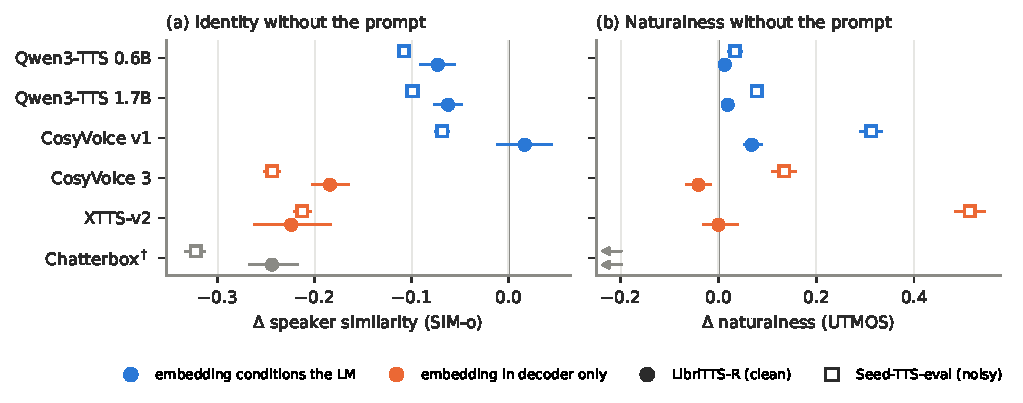
\includegraphics[width=0.92\textwidth]{../figures/pathway_headline}
  \caption{Effect of removing prompt-level conditioning (x-vector only minus full), speaker-level means with 95\% bootstrap CIs.
  (a)~Systems whose language model receives the speaker embedding (blue) keep most identity; systems that inject it only into the acoustic decoder (orange) lose most of it.
  (b)~Predicted naturalness rises most on the noisy Seed-TTS-eval prompts (squares).
  $^\dagger$Chatterbox stops producing intelligible speech without its prompt (UTMOS $-1.8$, off-scale).}
  \label{fig:headline}
\end{figure*}

\subsection{Across systems: an LM site helps identity survive}
\label{sec:identity}

Figure~\ref{fig:headline}a shows the change in SIM-o when the prompt is removed.
In the two systems whose language model receives the embedding and that still synthesise intelligible speech, identity largely survives: Qwen3-TTS loses 0.062--0.073 on LibriTTS-R and 0.099--0.108 on Seed-TTS-eval at both sizes, and CosyVoice loses nothing on LibriTTS-R ($+0.017$, n.s.) and 0.068 on Seed-TTS-eval.
In the two systems that inject the embedding only into the decoder, losses are two to three times larger: CosyVoice~3 loses 0.184 and 0.244, and XTTS-v2 0.224 and 0.213 (all $p_\text{Holm}{<}0.001$).
CosyVoice and CosyVoice~3 share a lineage and a front end and differ in whether the language model sees the embedding: the decoder-only successor loses 0.18 where its predecessor loses nothing (LibriTTS-R), and 3.6$\times$ as much on Seed-TTS-eval.
These systems differ in many other ways, so we test the role of each site directly in Section~\ref{sec:factorial}.
Chatterbox is the exception: although its language model receives an embedding, it does not produce intelligible speech without its speech prompt (WER 96--98\%), so the embedding alone is outside its operating regime.
With the prompt, WER is 1.7--5.9\% for all systems, and removing it leaves WER unchanged except for Chatterbox.

\subsection{Within CosyVoice: identity is split across sites}
\label{sec:factorial}

CosyVoice injects the same CAM++ embedding into both its language model and its flow decoder, so we can switch each site off (by zeroing the embedding, which both modules L2-normalise) independently of the prompt, keeping everything else fixed.
Table~\ref{tab:factorial} shows the 2$\times$2$\times$2 factorial on all LibriTTS-R cells and 300 Seed-TTS-eval items.
Without the prompt, both sites carry identity: removing the language-model embedding costs 0.113 SIM-o on LibriTTS-R (0.092 on Seed-TTS-eval), removing the decoder embedding costs 0.201 (0.181), and removing both costs 0.310 (0.272), close to the sum, leaving SIM-o near the 0.14 floor of an unconditioned voice.
With the prompt, the picture changes: removing the language-model embedding no longer matters ($-0.010$ and $-0.008$, n.s.), while removing the decoder embedding still costs 0.070 (0.057).
The prompt therefore substitutes for the embedding at the language model, where both are context for token generation, but not at the decoder.
This is the within-model counterpart of the cross-system pattern: relative to its full condition, CosyVoice's prompt-free SIM-o changes by $+0.017$ with both sites on (reproducing Section~\ref{sec:identity}) but by $-0.096$ with only the decoder site, moving towards its decoder-only successor ($-0.184$).

\begin{table}[t]
\centering
\caption{CosyVoice embedding-site factorial: SIM-o (speaker-level means) for each combination of prompt, language-model (LM) and decoder (flow) embedding. LibriTTS-R: 34 speakers $\times$ 5 targets $\times$ 3 seeds; Seed-TTS-eval: 300 items. Differences from the all-on cell within each prompt condition are significant at $p{<}10^{-8}$ unless marked n.s.}
\label{tab:factorial}
\small
\setlength{\tabcolsep}{4pt}
\resizebox{\columnwidth}{!}{%
\begin{tabular}{ccc|cc}
\toprule
\textbf{Prompt} & \textbf{LM emb.} & \textbf{Flow emb.} & \textbf{LibriTTS-R} & \textbf{Seed-TTS-eval} \\
\midrule
on  & on  & on  & 0.436 & 0.465 \\
on  & off & on  & 0.426 \scriptsize{(n.s.)} & 0.457 \scriptsize{(n.s.)} \\
on  & on  & off & 0.366 & 0.408 \\
on  & off & off & 0.333 & 0.387 \\
\midrule
off & on  & on  & 0.453 & 0.412 \\
off & off & on  & 0.340 & 0.320 \\
off & on  & off & 0.252 & 0.231 \\
off & off & off & 0.142 & 0.140 \\
\bottomrule
\end{tabular}%
}
\end{table}

\subsection{Prompts transfer recording conditions}
\label{sec:recording}

Figure~\ref{fig:headline}b shows that removing the prompt changes predicted naturalness little on clean LibriTTS-R ($-0.04$ to $+0.07$ for the systems that still work) but raises it on the noisier Seed-TTS-eval prompts in every such system: $+0.03$ and $+0.08$ for the two Qwen3-TTS sizes, $+0.13$ for CosyVoice~3, $+0.31$ for CosyVoice and $+0.51$ for XTTS-v2 (all $p_\text{Holm}{<}0.001$).
Two further observations indicate that the prompt carries recording-specific detail.
First, with the prompt, every system's output is closer to the specific prompt recording than to another recording of the same speaker, and removing the prompt shrinks this gap (SIM-p minus SIM-o) by 0.010--0.053 in all twelve system--dataset pairs (CI excludes zero in eleven).
Second, once the prompt is removed, XTTS-v2's output on Seed-TTS-eval is as similar to a held-out recording as to the prompt (gap 0.001): nothing recording-specific remains.
The naturalness gain from dropping the prompt is therefore largely a gain from \emph{not} copying a poor recording, rather than an intrinsic property of embedding conditioning.
A caution applies to the metric itself: in the CosyVoice factorial, removing \emph{all} speaker information raises predicted naturalness on Seed-TTS-eval from 4.04 to 4.35, so UTMOS also rewards generic voices, and naturalness gains that coincide with identity loss should not be read as better cloning.

\subsection{More references help identity, not naturalness}
\label{sec:refcount}

Table~\ref{tab:refcount} compares three references with one.
For Qwen3-TTS and CosyVoice~3, three references raise SIM-o by 0.022--0.044 in both routes, whether concatenated into the prompt or averaged as embeddings ($p{<}0.005$ for every system and route), and change naturalness by at most 0.02.
The prompt-only F5-TTS instead degrades with a three-reference prompt (SIM-o $-0.126$, UTMOS $-0.72$), consistent with prompt length being a trained-for property~\cite{megatts2}.

\begin{table}[t]
\centering
\caption{Three references minus one (LibriTTS-R, 34 speakers; speaker-level, pooled over selection strategy). $^\ast$\,$p{<}0.005$.}
\label{tab:refcount}
\small
\setlength{\tabcolsep}{4pt}
\begin{tabular}{llcc}
\toprule
\textbf{System} & \textbf{Route} & $\Delta$\textbf{SIM-o} & $\Delta$\textbf{UTMOS} \\
\midrule
Qwen3-TTS 0.6B & prompt (concat) & $+$0.043$^\ast$ & $-$0.008 \\
               & x-vector (avg)  & $+$0.036$^\ast$ & $-$0.003 \\
Qwen3-TTS 1.7B & prompt (concat) & $+$0.022$^\ast$ & $-$0.018$^\ast$ \\
               & x-vector (avg)  & $+$0.028$^\ast$ & $-$0.001 \\
CosyVoice~3    & prompt (concat) & $+$0.044$^\ast$ & $+$0.015 \\
               & x-vector (avg)  & $+$0.031$^\ast$ & $+$0.013 \\
F5-TTS         & prompt (concat) & $-$0.126$^\ast$ & $-$0.722$^\ast$ \\
\bottomrule
\end{tabular}
\end{table}

%----------------------------------------------------------------------
\section{Discussion and Conclusion}
\label{sec:conclusion}
%----------------------------------------------------------------------

The acoustic prompt and the speaker embedding are not redundant copies of the same information, and neither is the embedding at different depths of the model.
Within CosyVoice, the language-model and decoder sites each carry part of the speaker's identity and their contributions add; the prompt can replace the embedding at the language model, where both act as context for token generation, but it cannot replace the decoder's embedding.
Across systems, this explains why models that condition the language model as well as the decoder keep more identity when the prompt is removed, and it implies a design trade-off that recent systems have made implicitly: moving the embedding out of the language model, as CosyVoice~2/3 did~\cite{chen2026bottleneck}, makes identity more dependent on the prompt, with consequences for prompt-free, privacy-preserving or cross-lingual cloning.
Conversely, because identity survives from the embedding alone, speaker embeddings should be treated as identity-bearing, sensitive data.
The prompt, in turn, also carries the recording: noisy prompts are reproduced, so the naturalness benefit of embedding-only conditioning grows with prompt noise, although predicted naturalness also rises when identity is lost.
For practitioners, the conditioning route should be chosen per system and per recording quality, and when extra references are available, three references give a small, reliable gain in similarity in either route.

\textbf{Limitations.}
The causal factorial covers one model; the cross-system pattern rests on four working systems, and each system's prompt removal is a different intervention.
Zeroing an embedding leaves the downstream affine bias, a standard but not the only possible ablation.
All effects are measured with automatic metrics; a paired listening test is planned.
We evaluate English only, Seed-TTS-eval with a single seed, and for XTTS-v2 the removed latents are replaced by a held-out-speaker mean rather than deleted.

\section*{Generative AI Use Disclosure}
A generative AI coding assistant was used for experiment scripting and manuscript preparation.
All results, analysis, and scientific claims were verified by the authors.

\bibliographystyle{IEEEtran}
\bibliography{refs}

\end{document}
